\documentclass[a4paper,fleqn]{cas-sc}

\usepackage{graphicx}
\usepackage{subfigure}
\usepackage{amsfonts}
\usepackage{amsmath}
\usepackage{amssymb}
\usepackage{siunitx}
\sisetup{separate-uncertainty=true, per-mode=symbol}
\usepackage{indentfirst}
\usepackage{setspace}
\usepackage{lineno}
\usepackage[numbers]{natbib}
\pdfstringdefDisableCommands{%
  \def\corref#1{}%
  \def\fnref#1{}%
}


\begin{document}
\let\WriteBookmarks\relax

\shorttitle{Particle dynamics during slow resonant extraction}
\shortauthors{C.S. Park}
% Suppress the class's empty ORCID footnote; restore if an ORCID is supplied.
\let\printorcid\relax

\title [mode = title] {Particle dynamics during third-integer resonant extraction for Mu2e}
\author[1,2]{Chong Shik Park\corref{cor1}\fnref{fn1}}
\ead{kuphy@korea.ac.kr}
\cortext[cor1]{Corresponding author}
\fntext[fn1]{Formerly affiliated with Fermi National Accelerator Laboratory}

\affiliation[1]{organization={Department of Accelerator Science, Korea University},
%addressline={2511 Sejong-ro},
city={Sejong},
postcode={30019},
country={Republic of Korea}}

\affiliation[2]{organization={Accelerator Research Center, Korea University},
%addressline={2511 Sejong-ro},
city={Sejong},
postcode={30019},
country={Republic of Korea}}


\begin{abstract}
We investigate particle dynamics relevant to spill regulation and beam loss during third-integer resonant extraction from the Fermilab Delivery Ring for Mu2e. Multiparticle tracking with Synergia2 is combined with a reduced model based on the Kobayashi Hamiltonian and with MARS transport through the extraction channel. Radio-frequency knockout (RFKO) feedback reduces ripple-driven spill modulation in the simulated cases, although residual spikes remain. Tune-step studies at three stages of extraction show that transit times depend strongly on the initial phase-space coordinates and increase near the unstable fixed points. The reduced model reproduces the main trends but differs from the full tracking calculation near the separatrix. Tracking a MARS-generated scattered-particle sample identifies losses in the extraction channel and at downstream ring apertures; approximately 43\% of that sample is lost in the modeled ring. Separate RFKO studies show weak emittance growth and appreciable centroid motion at zero chromaticity, whereas nonzero chromaticity promotes emittance growth and suppresses coherent centroid motion. These results clarify the particle response relevant to spill feedback and identify the modeling and validation needed for quantitative predictions.
\end{abstract}

\begin{keywords}
Mu2e \sep Resonant extraction \sep Spill regulation \sep Beam dynamics \sep Radio-frequency knockout
\end{keywords}

\maketitle
\hypersetup{pdfauthor={Chong Shik Park}}

% Review layout: retain line numbers and double spacing for editorial review.
\doublespacing
\linenumbers


%%%%%%%%%%%%%%%%%%%%%%%%%%%%%%%%%%%%%%%%%%%%%%%%%%
\section{\label{sec:intro}Introduction}

Slow resonant extraction from the Delivery Ring is part of the proton-delivery scheme for the Mu2e experiment at Fermilab~\cite{tdr}. Harmonic sextupoles excite the third-integer resonance, and a ramp of the tune-control quadrupoles moves the beam toward resonance. Previous Synergia2 simulations examined a piecewise linear tune ramp, septum alignment, and local orbit corrections for this extraction scheme~\cite{mu2e}. The present study uses the design parameters in Table~\ref{table:param} to investigate the particle dynamics underlying spill feedback, transit-time distributions, and the subsequent transport of particles scattered in the septa. These parameters describe the simulated configuration rather than an operational measurement.


\begin{table}[width=\linewidth,cols=3,pos=htbp]
  \caption{\label{table:param}Beam and machine parameters used in the simulations. The mean number of protons per extracted pulse is $10^{12}/31{,}795 \simeq 3.15\times10^{7}$, assuming one extracted pulse per revolution.}
  \begin{tabular*}{\tblwidth}{@{} LRR@{}}
    \toprule
    Parameter & Value & Unit \\
    \midrule
    Beam momentum & 8.886 & $\mathrm{GeV}/c$ \\
    Protons per spill & $1.0\times10^{12}$ & \\
    Magnetic rigidity, $B\rho$ & 29.650 & $\mathrm{T\,m}$ \\
    rms bunch length & 40 & ns \\
    95\% normalized emittance & 20 & $\pi\,\mathrm{mm\,mrad}$ \\
    Ring circumference & 505.283 & m \\
    Horizontal resonance tune, $\nu_{\mathrm{res}}$ & $29/3$ & \\
    Bare tunes, $(\nu_{x0},\nu_{y0})$ & $(9.65,9.78)$ & \\
    Relative momentum spread, $\Delta p/p$ & 0.0016 & \\
    Spill duration & 54 & ms \\
    Turns per spill & 31,795 & \\
    Mean protons per extracted pulse & $3.15\times10^{7}$ & \\
    RF harmonic number & 4 & \\
    RF frequency & 2.36 & MHz \\
    Peak RF voltage & 10 & kV \\
    \bottomrule
  \end{tabular*}
\end{table}


The Hardt condition aligns the outgoing separatrices for different momenta and thereby reduces the momentum dependence of the extracted-beam angle~\cite{hardt,pullia,pimms}. The dispersion-free extraction region in the Delivery Ring constrains this approach. Local orbit corrections and septum alignment have therefore been studied to control the beam position and angle at the septum~\cite{mu2e}. Those corrections provide context for the present work; their optimization is not repeated here.

Maintaining a uniform spill requires control of both the average extraction rate and fluctuations driven by magnet errors or power-supply ripple. Radio-frequency knockout (RFKO) provides transverse excitation that can be adjusted in response to the measured spill rate~\cite{HB10,ipac11}. Its feedback response depends on the delay between excitation, escape from the stable region, and arrival at the septum. We study this delay using tune-step tracking calculations and compare the results with a reduced resonance model.

Aperture-based tracking identifies particles that intercept extraction-channel components but does not, by itself, describe their subsequent scattering. We therefore combine Synergia2 tracking with MARS transport through the septa and downstream extraction elements~\cite{mars1,mars2}. The returned scattered-particle sample is then tracked around the ring to locate subsequent losses. A separate RFKO study examines how chromaticity affects the balance between coherent centroid motion and emittance growth.

The calculations use complementary descriptions of the beam. Synergia2 provides multiparticle tracking with space charge~\cite{synergia2}; the Kobayashi Hamiltonian isolates horizontal resonance dynamics without space charge or detailed extraction-channel geometry; and MARS models particle interactions with material. Comparisons between these descriptions are used to interpret the dynamics, rather than to establish a complete validation of the loss or feedback models.

Section~\ref{sec:rfko1} describes the simulated RFKO feedback. Section~\ref{sec:tracking} presents the reduced Hamiltonian, transit-time calculations, and scattered-particle tracking. Section~\ref{sec:rfko} examines RFKO-driven emittance growth and action distributions, and Sec.~\ref{sec:conclusion} summarizes the results and their limitations.


%%%%%%%%%%%%%%%%%%%%%%%%%%%%%%%%%%%%%%%%%%%%%%%%%%
\section{\label{sec:rfko1}Spill regulation with RFKO feedback}

A piecewise linear ramp of the tune-control quadrupoles can maintain an approximately constant average extraction rate~\cite{mu2e}. Magnet errors and power-supply ripple can nevertheless produce fluctuations about that average. The RFKO system applies a transverse RF kick near the horizontal betatron frequency to increase particle amplitudes and assist their passage across the separatrix~\cite{HB10,ipac11}.

The proposed feedback loop comprises an RFKO kicker, a spill monitor, and a controller. A wall-current monitor in the external beamline supplies the extracted-beam signal used to adjust the kicker amplitude~\cite{wcm}. The simulated control scheme uses a spill signal accumulated over approximately 100 turns, corresponding to about $0.17\,\mathrm{ms}$. This averaging interval and the particle transit-time distribution both contribute to the effective response time.

The RFKO center frequency follows the betatron frequency associated with the ramped machine tune. Frequency modulation broadens the excitation to cover the chromatic tune spread. In the extraction simulations, the horizontal chromaticity is set to $C_x=d\nu_x/d\delta=1.0$, where $\delta=(p-p_0)/p_0$, using chromaticity-correction sextupoles. The incoherent space-charge tune spread alone need not provide the phase mixing required for efficient emittance growth under dipole excitation~\cite{ipac11}; this distinction is examined further in Sec.~\ref{sec:rfko}.

The excitation uses a linear frequency chirp with a sweep duration of 100 turns. Repeating an identical sweep produces discrete spectral lines. Randomizing the phase at the start of each sweep reduces this periodic structure and broadens the excitation spectrum.

To test the response to a controlled disturbance, a sinusoidal ripple at $60\,\mathrm{Hz}$ is applied to the quadrupole strengths. The fractional modulation is specified as $\pm0.5\%$ about the nominal strengths. It produces pronounced spill modulation, including components at harmonics of the applied ripple frequency.
% AUTHOR CHECK: the original draft also called this value "peak-to-peak".
% Confirm whether the simulation used a 0.5% amplitude or a 0.5% peak-to-peak ripple.

\begin{figure}[pos=!tbp]
  \centering
  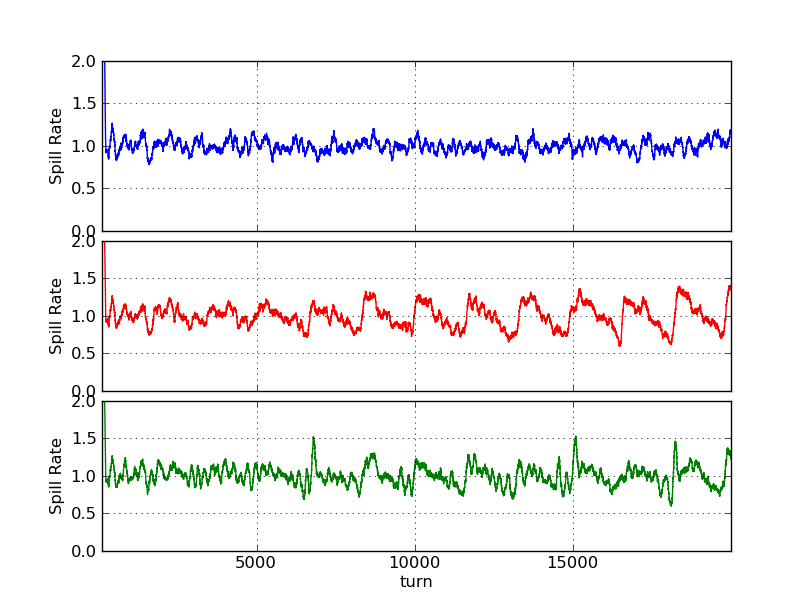
\includegraphics[width=.9\textwidth]{img/fig9.png}
  \caption{\label{fig:fig9}Normalized spill rate for three simulated configurations: no ripple and no feedback (top), quadrupole ripple without feedback (middle), and quadrupole ripple with RFKO feedback (bottom). Feedback reduces the visible ripple-driven modulation, although residual spikes remain.}
\end{figure}

Controllers based on proportional--integral--derivative feedback were investigated~\cite{pid}. Proportional-only control produced large spill oscillations, consistent with excessive correction in the presence of a delayed beam response. Among the tested configurations, a time-dependent proportional gain combined with a constant derivative gain gave the most favorable behavior. The result shown here therefore uses proportional--derivative control, without an integral term.

Figure~\ref{fig:fig9} shows a qualitative reduction in ripple-driven modulation with feedback. The remaining spikes indicate that the tested controller does not eliminate all fluctuations. The traces do not establish a numerical suppression factor, a stability margin, or an optimum set of gains. An integral term could be investigated to reduce steady-state error, but its effect on stability and spill fluctuations has not been demonstrated here.

%%%%%%%%%%%%%%%%%%%%%%%%%%%%%%%%%%%%%%%%%%%%%%%%%%%%%%%%%

\section{\label{sec:tracking}Particle tracking simulations}

\subsection{\label{sec:model}Reduced resonance model and Kobayashi Hamiltonian}

Let $x$ be the horizontal displacement from the reference orbit, $x'=dx/ds$ the horizontal angle, and $\alpha$ and $\beta$ the horizontal Twiss parameters at the observation point. Define the normalized coordinates
\begin{equation}
 X=\frac{x}{\sqrt{\beta}},\qquad
 X'=\frac{\alpha x+\beta x'}{\sqrt{\beta}},\qquad
 a=\frac{X+iX'}{\sqrt{2}}.
 \label{eqn:coordinates}
\end{equation}
Here $X'$ denotes the normalized momentum coordinate, not $dX/ds$. In the resonance frame, the leading-order third-integer Hamiltonian is~\cite{preliminary}
\begin{equation}
 H=\Delta\nu\,a^*a-ig a^3+ig^*(a^*)^3+\cdots,
 \label{eqn:hamiltonian1}
\end{equation}
where $\Delta\nu=\nu_x-29/3$ and $g$ is the complex resonance-driving coefficient determined by the sextupole strengths and phases. The cubic terms are complex conjugates, so their sum is real. Higher-order terms are neglected in the reduced model.

Writing $g=|g|e^{i\Psi}$ and substituting Eq.~\eqref{eqn:coordinates} gives
\begin{equation}
\begin{split}
 H={}&\frac{\Delta\nu}{2}(X^2+X'^2)\\
 &+\frac{|g|}{\sqrt{2}}\left[(X^3-3XX'^2)\sin\Psi
             +(3X^2X'-X'^3)\cos\Psi\right].
\end{split}
 \label{eqn:hamiltonian2}
\end{equation}
For the separatrix orientation used here, set $\Psi=\pi$. Multiplying Eq.~\eqref{eqn:hamiltonian2} by $6\pi$ gives the three-turn Kobayashi Hamiltonian~\cite{kobayashi},
\begin{equation}
 H_K=\frac{\epsilon}{2}(X^2+X'^2)
       +\frac{S}{4}(3X^2X'-X'^3),
 \label{eqn:kobayashi}
\end{equation}
with $\epsilon=6\pi\Delta\nu$ and $S=-12\sqrt{2}\pi|g|$. This sign of $S$ follows from the specified phase $\Psi=\pi$. For the below-resonance setting $\Delta\nu<0$ considered here, it agrees with $12\sqrt{2}\pi|g|\,\mathrm{sgn}(\Delta\nu)$; the latter is not a general definition for a fixed separatrix orientation.

The quadratic term describes linear motion, which is circular in normalized phase space. Below resonance, this motion is counterclockwise with the present coordinate convention. The cubic term creates a triangular stable region bounded by a separatrix, with hyperbolic unstable fixed points at its vertices. Particles outside the stable region can move along the outgoing branches toward the septum.

Introducing the continuous turn variable $\tau=n/3$, where $n$ is the number of revolutions, Hamilton's equations become
\begin{equation}
 \begin{split}
  \frac{dX}{d\tau} & = \frac{\partial H_{K}}{\partial X^{\prime}}
                  = \epsilon X^{\prime} + \frac{3}{4} S
                    \left(
                      X^{2} - X^{\prime 2}
                    \right), \\
  \frac{dX^{\prime}}{d\tau} & = - \frac{\partial H_{K}}{\partial X}
                           = - \epsilon X - \frac{3}{2} S X X^{\prime}.
 \end{split}
\label{eqn:motion}
\end{equation}
One unit of $\tau$ corresponds to three turns; the physical elapsed time is $t_{\mathrm{phys}}=3T_{\mathrm{rev}}\tau$. The momentum and circumference in Table~\ref{table:param} give $T_{\mathrm{rev}}\simeq1.69\,\mu\mathrm{s}$, consistent with $54\,\mathrm{ms}$ over approximately 31,795 turns. The three-turn interval is short compared with the spill duration, but this separation of timescales alone does not guarantee adiabatic motion near a separatrix. The tune steps used below are explicitly nonadiabatic changes followed by tracking at fixed quadrupole strengths.

The reduced model retains horizontal resonance dynamics but omits space charge and detailed lattice and extraction-channel effects. It is used to interpret the Synergia2 trajectories and their transit times. Agreement in qualitative features does not by itself validate the full tracking or scattering calculation.


\subsection{\label{sec:arrival}Transit-time distributions}

The transit time is the interval between a particle becoming unstable and reaching the septum field region~\cite{pullia}. In the diagnostic used here, elapsed time is measured from an imposed tune step. The resulting response includes particles already in transit as well as particles made unstable by the step, unless these populations are explicitly separated.

Analytical treatments based on the Kobayashi Hamiltonian describe transit times for fixed or slowly varying resonance conditions~\cite{pullia}. Near an unstable fixed point, the phase-space velocity becomes small and escape can take many turns. This produces a strong dependence on initial conditions and long transit-time tails. Such behavior reflects slow passage near a hyperbolic point, rather than trapping by a stable fixed point.

\begin{figure}[pos=!tbp]
  \centering
  \subfigure[Beam intensities]{
    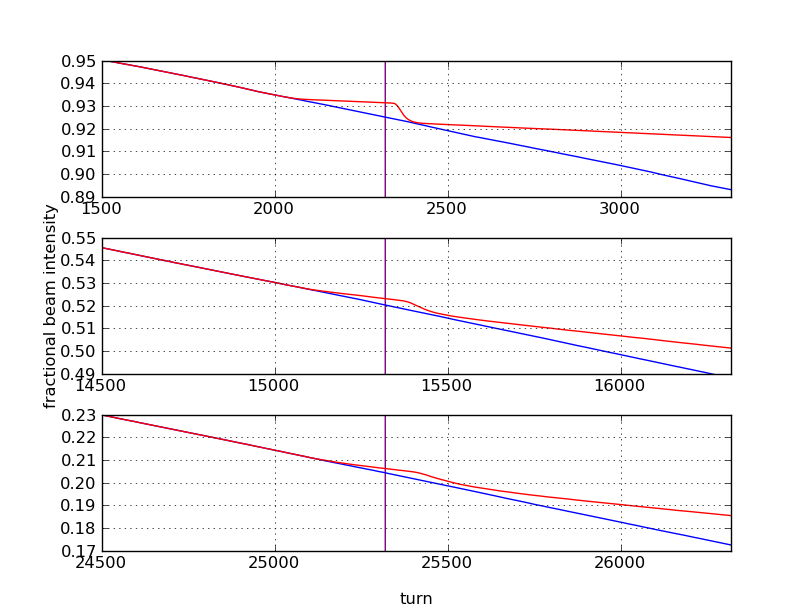
\includegraphics[width=.45\textwidth]{img/fig_arrival1a}
    \label{fig:arrival1a}}
  \subfigure[Normalized spill intensity]{
    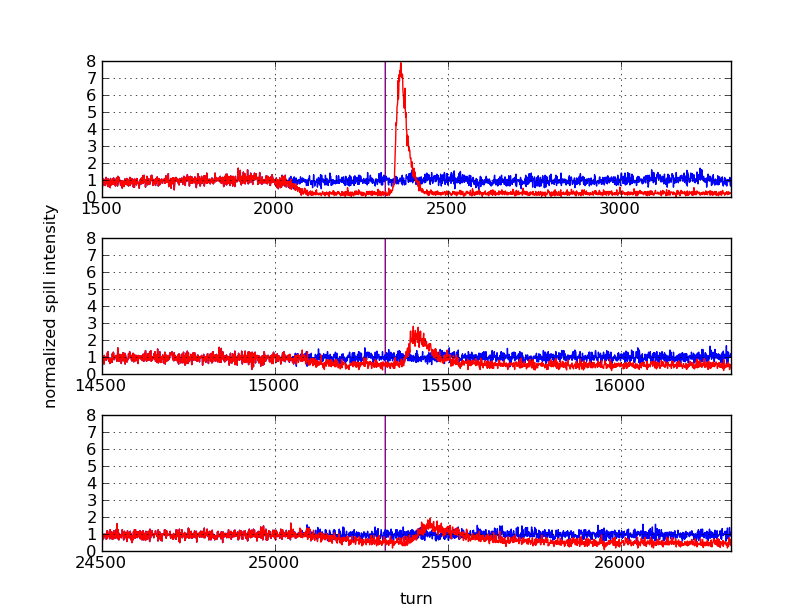
\includegraphics[width=.45\textwidth]{img/fig_arrival1b}
    \label{fig:arrival1b}}
  \caption{\label{fig:arrival1}Tune-step diagnostic at early (top), middle (center), and late (bottom) stages of extraction. Panel (a) shows the circulating-beam fraction and panel (b) the normalized spill intensity. Blue curves use the uninterrupted ramp; red curves use the paused-and-restored ramp. Purple vertical lines mark restoration of the quadrupole strengths to the values of the uninterrupted ramp at that turn.}
\end{figure}

The Synergia2 calculation starts with $5\times10^5$ macroparticles and the parameters in Table~\ref{table:param}. At a selected turn, the tune-quadrupole ramp is paused for approximately 300 turns, or about 1\% of the spill duration. The strengths are then stepped to the values that the uninterrupted ramp would have reached at that turn and held for a further observation interval of approximately 500 turns. The step reduces the stable region and releases a population near its boundary. This procedure probes the extraction response to a finite tune change; it is not a measurement of the feedback-loop transfer function.

The pauses begin at turns 2,000, 15,000, and 25,000, representing early, middle, and late extraction. The changing separatrix size and its distance from the septum can affect transit times. Using the same initial macroparticle population at the three stages allows these trends to be compared, although the number of particles contributing to each distribution differs and no statistical-convergence study is presented.

Figure~\ref{fig:arrival1a} shows the evolution of the circulating-beam fraction. The uninterrupted ramp produces a nearly steady decrease in beam intensity. Pausing the ramp slows extraction, and the subsequent tune step produces an additional decrease in circulating intensity. The corresponding normalized spill traces in Fig.~\ref{fig:arrival1b} show a pronounced burst in the early-stage case and a weaker, broader response at the later stages. Continued extraction during a pause is consistent with particles already traveling toward the septum and, in the full calculation, with evolving collective dynamics. The traces alone do not isolate the contributions of these effects.

\begin{figure}[pos=!tbp]
  \centering
  \subfigure[Turn 2,000]{
    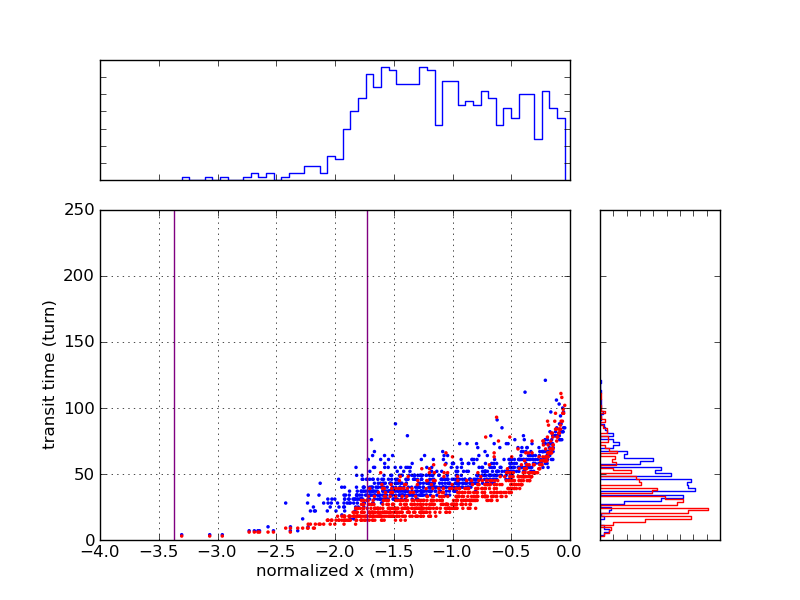
\includegraphics[width=.47\textwidth]{img/fig_arrival2a}
    \label{fig:arrival2a}}
  \subfigure[Turn 15,000]{
    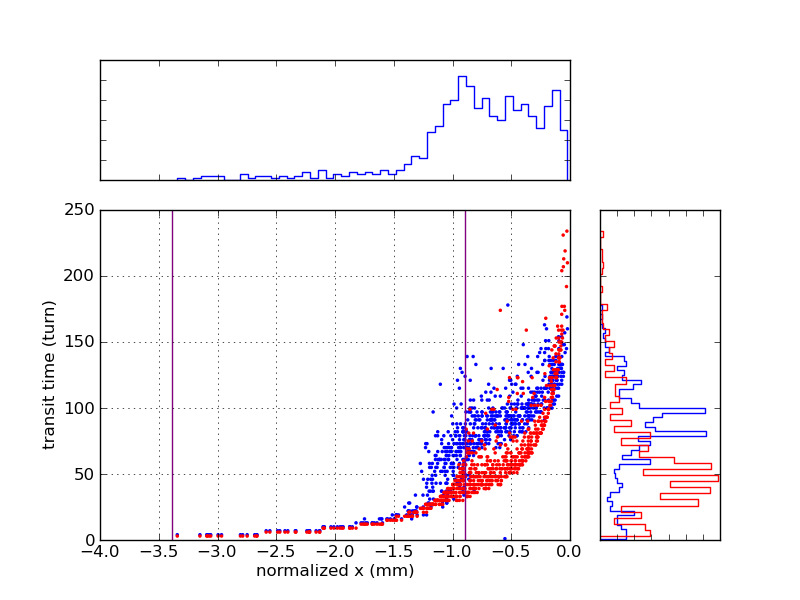
\includegraphics[width=.47\textwidth]{img/fig_arrival2b}
    \label{fig:arrival2b}}
  \par\medskip
  \subfigure[Turn 25,000]{
    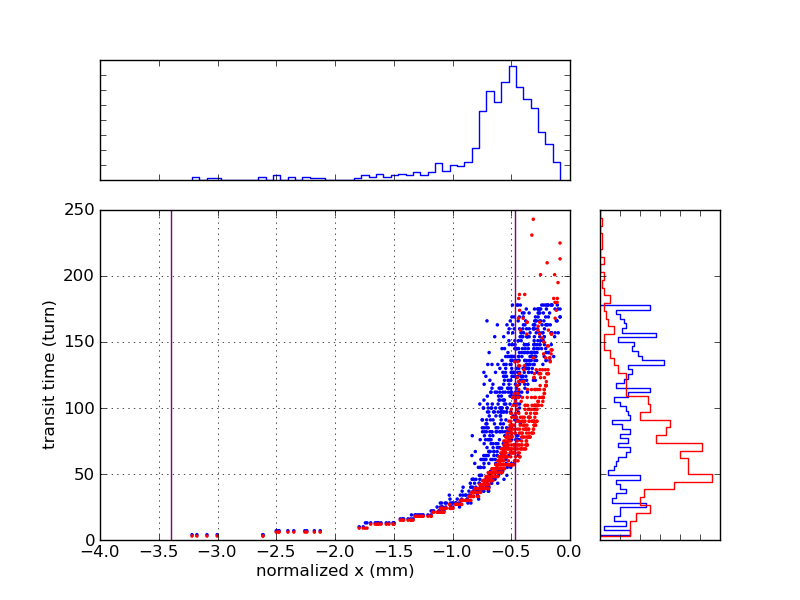
\includegraphics[width=.47\textwidth]{img/fig_arrival2c}
    \label{fig:arrival2c}}
  \caption{\label{fig:arrival2}Transit time versus initial horizontal coordinate for the early, middle, and late tune-step cases. Blue and red markers denote Synergia2 and reduced-model RK4 tracking, respectively. Marginal histograms show the coordinate and transit-time distributions. The left vertical line marks the septum position; the right line marks the horizontal coordinate of the leftmost unstable fixed point. Coordinate units and normalization follow the original simulation plots.}
\end{figure}

For comparison, Eq.~\eqref{eqn:motion} is integrated with a fourth-order Runge--Kutta (RK4) method. The reduced-model trajectories use the same initial particle coordinates as the Synergia2 sample, and the effective resonance parameters are evaluated at the restored quadrupole settings. Space charge is omitted in the reduced model. The continuous variable $\tau$ must be converted to turns when comparing transit times; observing trajectories every three turns does not prescribe the numerical integration step.

Figure~\ref{fig:arrival2} compares individual-particle transit times and their marginal distributions. Both calculations show short transit times for particles starting close to the septum along the outgoing branch, with increasing times for starting coordinates nearer the unstable fixed point. Away from the short-transit region, the full tracking result has a broader distribution and differs systematically from the reduced model.

Transit time depends on the full initial phase-space coordinates and resonance parameters; it is not generally inversely proportional to the perpendicular distance from a separatrix. Slow escape near a hyperbolic fixed point accounts qualitatively for the long transit times in both calculations. Space charge can change individual trajectories and the effective resonance conditions in Synergia2. However, the comparison also changes the lattice description and other model details, so the observed differences cannot be attributed uniquely to space charge without a matched calculation in which space charge alone is switched off.


\subsection{\label{sec:beamloss}Tracking of particles scattered at the septum}

Particles moving along an outgoing separatrix branch enter the electrostatic septum field and receive a deflection toward the extraction line. The modeled channel contains two electrostatic septa with $50\,\mu\mathrm{m}$ foils. Finite foil thickness and extent allow some particles to intercept material and scatter. The aperture-based Synergia2 calculations reported an interception fraction below approximately 2\% for the studied configurations. An interception fraction is distinct from the fraction ultimately lost after scattering and further transport.

In the aperture treatment used here, a particle that intercepts a septum component is removed from the primary tracking sample. This does not determine its subsequent fate. A scattered particle may return to the field-free region, receive a partial electrostatic kick, be extracted, or be lost at another aperture. MARS transport is used to resolve these alternatives through the extraction-channel geometry before selected scattered particles are returned to ring tracking.

\begin{figure}[pos=!tbp]
  \centering
  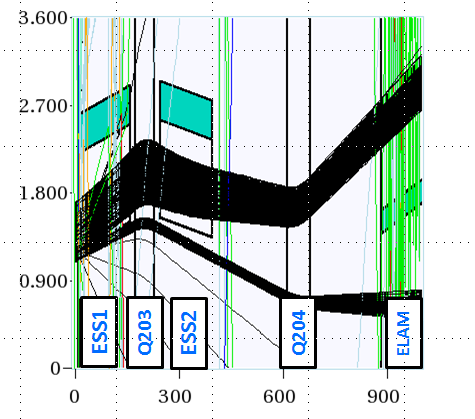
\includegraphics[width=.68\textwidth]{img/fig_beamloss1}
  \caption{\label{fig:beamloss1}MARS trajectories through the modeled extraction channel, showing ESS1, Q203, ESS2, Q204, and the Lambertson magnet (ELAM). The main black trajectories represent circulating (upper) and outgoing (lower) protons; other trajectories illustrate scattering and secondary-particle transport. The downstream C-magnet is outside the displayed region.}
\end{figure}

MARS models hadronic and electromagnetic interactions, including secondary-particle production~\cite{mars2}. Figure~\ref{fig:beamloss1} shows transport through the two electrostatic septa (ESS1 and ESS2), two quadrupoles (Q203 and Q204), and the Lambertson magnet (ELAM). The outgoing beam subsequently reaches the C-magnet. Separation of the circulating and outgoing beams begins at ESS1 and increases before ESS2. The displayed trajectories illustrate this separation but do not, by themselves, establish zero loss at ESS2.

The tracking workflow has three stages. First, a specialized Synergia2 aperture at ESS1 selects particles that hit the foil head or another entrance component, or whose calculated trajectories cross a septum plane inside the element. Second, these particles are transported by MARS from ESS1 through the extraction channel to the C-magnet, using the modeled foil thicknesses, widths, spacings, and materials~\cite{mars1}. Third, the scattered-particle output selected for further ring transport is used as input to Synergia2. The loss fraction below refers to this returned sample; it is not an inclusive count of all secondary species produced by MARS.

\begin{figure}[pos=!tbp]
  \centering
  \subfigure[Phase-space trajectories]{
    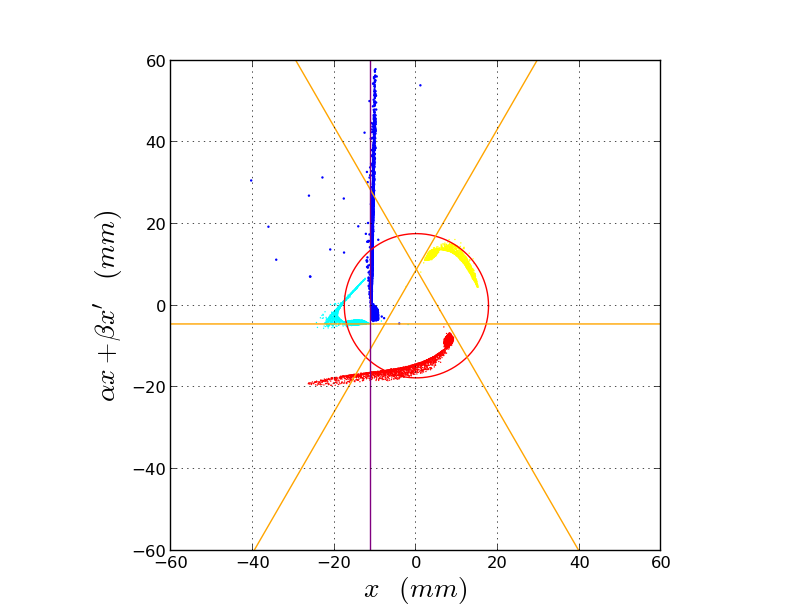
\includegraphics[width=.45\textwidth]{img/fig_beamloss2a}
    \label{fig:beamloss2a}}
  \subfigure[Loss locations]{
    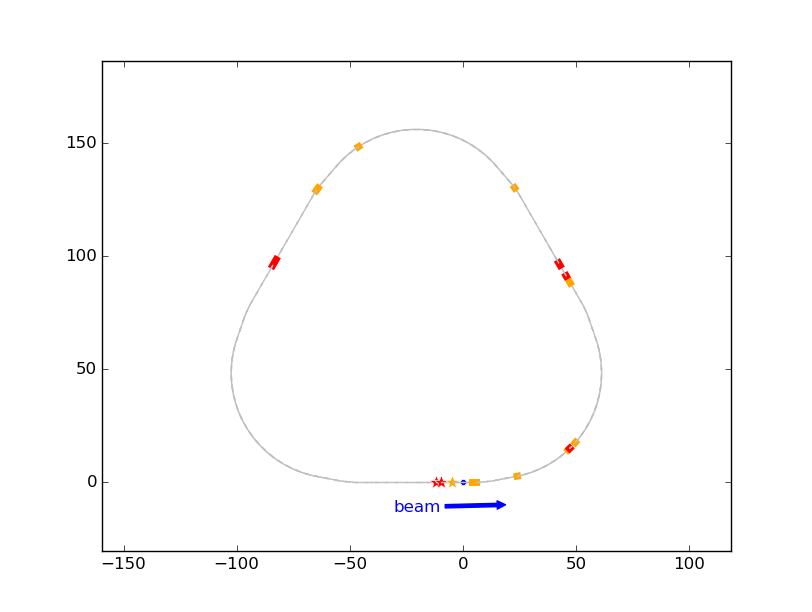
\includegraphics[width=.45\textwidth]{img/fig_beamloss2b}
    \label{fig:beamloss2b}}
  \caption{\label{fig:beamloss2}Synergia2 tracking of the returned scattered-particle sample. (a) Turn-by-turn distributions referred to ESS1, plotted in $(x,\,\alpha x+\beta x')$ coordinates. The initial sample is blue; subsequent turns are red, yellow, and cyan. (b) Locations of losses around the Delivery Ring. These coordinates in panel (a) retain a factor of $\sqrt{\beta}$ relative to $(X,X')$ in Eq.~\eqref{eqn:coordinates}.}
\end{figure}

Figure~\ref{fig:beamloss2a} shows the scattered-particle sample referred back from the C-magnet to ESS1 for comparison. The initial particles lie near the septum line at $x\simeq-11\,\mathrm{mm}$. Additional circulating particles are included as a visual reference and form the compact group near one end of the initial distribution. The next three turns populate the lower, right, and left regions of the plot. After three turns, many surviving particles have returned to the septum field region. Figure~\ref{fig:beamloss2b} locates losses near the septa, in the first arc, and near the middles of the straight sections. Approximately 43\% of the tracked scattered-particle sample is reported lost, with the remainder surviving to extraction. This conditional fraction cannot be combined with the initial interception estimate to obtain a total beam-loss fraction without consistent sample weights, selection criteria, and tracking endpoints.

\begin{figure}[pos=!tbp]
  \centering
  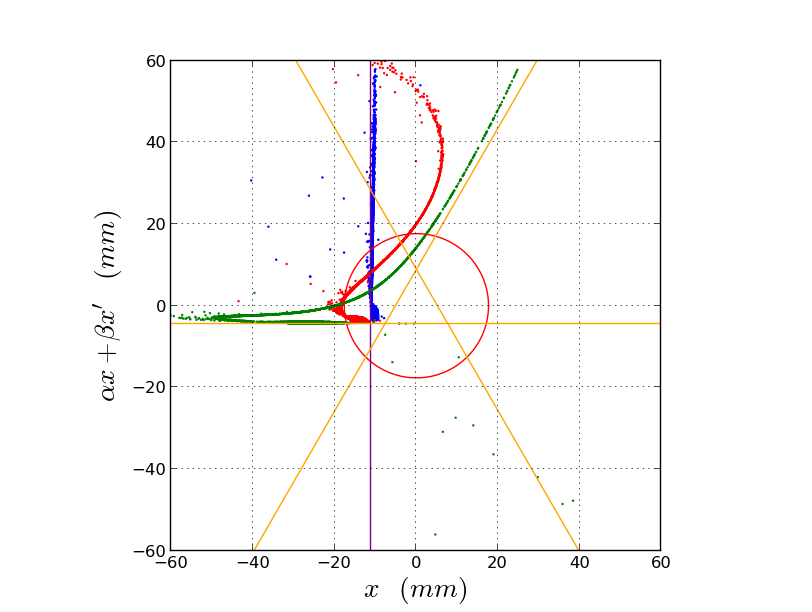
\includegraphics[width=.75\textwidth]{img/fig_beamloss3}
  \caption{\label{fig:beamloss3} Reduced-model trajectories sampled at turns 0 (blue), 3 (red), and 6 (green), shown in the same phase-space coordinates as Fig.~\ref{fig:beamloss2a}. The septum line is a reference only: extraction fields, material interactions, and particle removal are absent from this calculation.}
\end{figure}

Although the initial scattered-particle distribution is approximately aligned with the septum, its subsequent distributions are curved. After three turns, the added circulating-particle group follows the outgoing separatrix branch, whereas scattered particles can lie away from that branch. The distinction matters when interpreting the apparent shape of the combined distribution.

Figure~\ref{fig:beamloss3} illustrates this deformation using the reduced Hamiltonian. It omits the extraction fields and apertures, so trajectories continue beyond the reference septum line. Particles initially lying on a straight line generally have different Hamiltonian values and follow different level curves at different speeds. Their distribution therefore deforms after three and six turns. This behavior provides a qualitative explanation of phase-space shearing in the Synergia2 results, but it does not validate material scattering, aperture losses, or extraction efficiency.


\section{\label{sec:rfko}Effects of RFKO excitation on emittance and centroid motion}

\begin{figure}[pos=!tbp]
  \centering
  \subfigure[Horizontal emittance]{
    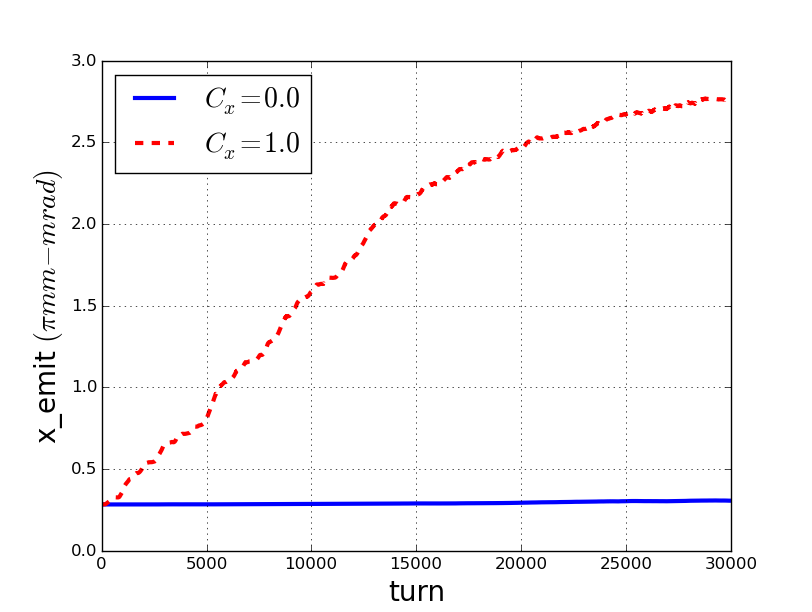
\includegraphics[width=.45\textwidth]{img/fig_rfko1a}
    \label{fig:rfko1a}}
  \subfigure[Beam-centroid motion]{
    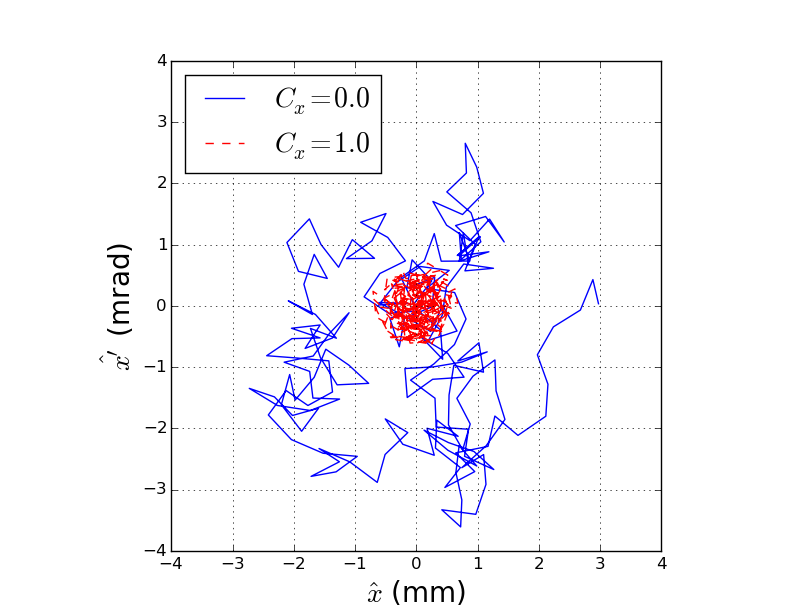
\includegraphics[width=.45\textwidth]{img/fig_rfko1b}
    \label{fig:rfko1b}}
  \caption{\label{fig:rfko1}RFKO excitation at $C_x=0$ (blue, solid) and $C_x=1$ (red, dashed). (a) Horizontal emittance versus turn. (b) Beam-centroid trajectories over 30,000 turns. Nonzero chromaticity produces greater emittance growth and smaller centroid excursions in these simulations.}
\end{figure}

The tune-quadrupole ramp drives the principal extraction process, while RFKO provides an additional means of regulating the spill. To separate the response to RFKO from the resonance-driven extraction dynamics, this section considers excitation at a fixed machine tune without the third-integer resonance drive. The quantities of interest are emittance, centroid motion, and the distribution of horizontal action.

Earlier simulations found effective excitation when the RFKO center frequency follows the machine tune and the modulation bandwidth is comparable to the chromatic tune spread~\cite{ipac11}. Dipole excitation can drive coherent motion without a corresponding increase in emittance about the beam centroid. A spread in betatron frequencies promotes phase mixing, allowing the excitation to increase the internal phase-space area. An incoherent space-charge tune spread does not necessarily provide the same mixing mechanism as chromaticity.

The horizontal machine tune is fixed at 9.65, and the resonance drive and tune ramp are disabled. The model includes space charge and uses a circular transverse aperture, specified in the original simulation as a $20\pi\,\mathrm{mm\,mrad}$ acceptance, to remove particles outside the accepted region. A linear chirp with randomized sweep phases supplies the RFKO excitation. Two horizontal chromaticities, $C_x=0$ and $C_x=1$, are compared. The assumed RFKO power is $500\,\mathrm{W}$, corresponding in the modeled kicker to an approximately $1\,\mu\mathrm{rad}$ horizontal kick.
% AUTHOR CHECK: supply the acceptance/action convention, chirp bandwidth in
% each case (including C_x=0), and kicker calibration from the simulation inputs.

Figure~\ref{fig:rfko1a} shows little emittance growth at $C_x=0$ and substantially greater growth at $C_x=1$. The centroid trajectories in Fig.~\ref{fig:rfko1b} show the complementary behavior: large coherent excursions at zero chromaticity and motion concentrated near the origin at nonzero chromaticity. These results are consistent with chromatic phase mixing converting the driven response into increased internal beam spread. They do not imply that the RFKO force is absent or decoupled from the particles at zero chromaticity.

\begin{figure}[pos=!tbp]
  \centering
  \subfigure[$C_{x} = 0.0$]{
    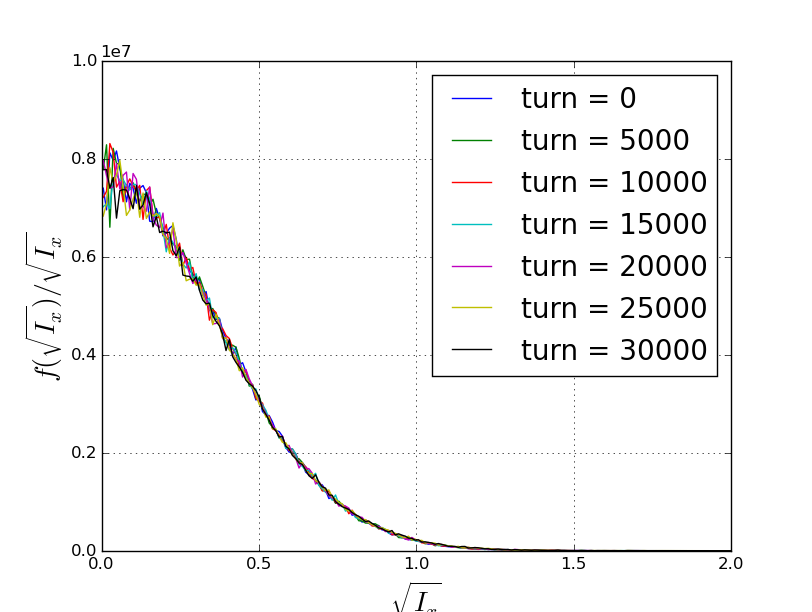
\includegraphics[width=.45\textwidth]{img/fig_rfko2a}
    \label{fig:rfko2a}}
  \subfigure[$C_{x} = 1.0$]{
    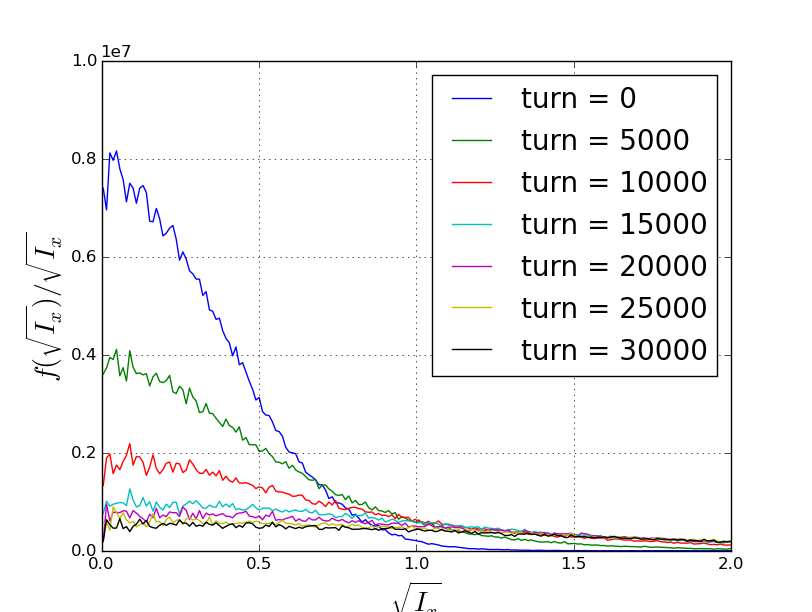
\includegraphics[width=.45\textwidth]{img/fig_rfko2b}
    \label{fig:rfko2b}}
  \caption{\label{fig:rfko2}Evolution of the plotted horizontal-action distributions, $f(\sqrt{I_x})/\sqrt{I_x}$ versus $\sqrt{I_x}$, at 5,000-turn intervals for (a) $C_x=0$ and (b) $C_x=1$. The original diagnostic normalization is retained. Particles outside the modeled aperture are removed, so changes in distribution height need not represent redistribution alone.}
\end{figure}

The action distributions in Fig.~\ref{fig:rfko2} remain approximately unchanged for $C_x=0$. At $C_x=1$, the low-action population decreases and the distribution broadens under continued excitation. Because the aperture removes particles, interpreting the distribution quantitatively also requires the surviving population and a fixed normalization convention. These calculations support the role of chromaticity in RFKO-driven emittance growth. Since the resonance drive is disabled in this test, they do not directly demonstrate transfer into an extraction resonance or quantify the resulting spill.


\section{\label{sec:conclusion}Conclusions}

The simulations examine three aspects of particle dynamics relevant to third-integer extraction for Mu2e: RFKO spill feedback, transit times following tune changes, and the fate of particles scattered in the extraction septa. The tested proportional--derivative controller reduces visible ripple-driven spill modulation, but residual spikes remain and a quantitative suppression metric has not been established.

Tune-step calculations at three stages of extraction show a strong dependence of transit time on initial phase-space coordinates, with long delays near unstable fixed points. The reduced Kobayashi model reproduces the main trends while differing from Synergia2 near the separatrix. Because the models differ in more than their treatment of space charge, matched tracking comparisons are needed to identify the source of those differences.

The combined Synergia2--MARS workflow locates subsequent losses of a scattered-particle sample in the extraction channel and elsewhere around the ring. The reported loss of approximately 43\% applies to that sample rather than to the full circulating beam. Reduced-model trajectories explain phase-space shearing qualitatively, without validating the scattering calculation. Separate RFKO tests show that nonzero chromaticity favors emittance growth and smaller centroid excursions, whereas zero chromaticity primarily produces coherent motion in the studied configuration.

These results provide a physical basis for refining spill feedback and loss modeling. Quantitative predictions require documented controller settings and latency, convergence checks for tracking and transit-time distributions, and a fully specified particle handoff between MARS and Synergia2. The present evidence supports these priorities without establishing final operational performance.



\section{\label{thanks}Acknowledgments}

This work was supported by the United States Department of Energy under contract DE-AC02-07CH11359 and the ComPASS project funded through the Scientific Discovery through Advanced Computing program in the DOE Office of High Energy Physics.


\clearpage
\begin{thebibliography}{99}

\bibitem{tdr}
L. Bartoszek et al. (Mu2e Collaboration), ``Mu2e Technical Design Report,'' FERMILAB-TM-2594 (2014), \href{https://arxiv.org/abs/1501.05241}{arXiv:1501.05241}.

\bibitem{mu2e}
C.S. Park, ``Tracking simulation of third-integer resonant extraction for Fermilab's Mu2e experiment,'' Nuclear Engineering and Technology \textbf{58} (2026) 104097, \href{https://doi.org/10.1016/j.net.2025.104097}{doi:10.1016/j.net.2025.104097}.

\bibitem{hardt}
  W. Hardt, ``Ultraslow Extraction out of LEAR,'' CERN Internal Note PS/DL/LEAR Note 81-6, 1981.

\bibitem{pullia}
M. Pullia, ``Detailed dynamics of slow extraction and its influence on transfer line design,'' Ph.D. thesis, Universit\'e Claude Bernard Lyon 1 (1999).

\bibitem{pimms}
PIMMS Study Group, ``Proton-Ion Medical Machine Study (PIMMS),'' Part I, CERN/PS 99-010 (DI) (1999); Part II, CERN/PS 2000-007 (DR) (2000).

\bibitem{HB10}
  V. Nagaslaev, J. Amundson, J. Johnstone, L. Michelotti, C.S. Park, S. Werkema, and M. Syphers, ``Third Integer Resonance Slow Extraction Scheme for a $\mu\to e$ Experiment at Fermilab,'' FERMILAB-CONF-10-395-AD (2010), contribution to HB2010.

\bibitem{ipac11}
V. Nagaslaev, J. Amundson, J. Johnstone, C.S. Park, and S. Werkema, ``Third Integer Resonance Slow Extraction Using RFKO at High Space Charge,'' in Proceedings of IPAC2011, San Sebasti\'an, Spain (2011), pp. 3559--3561, paper THPS058.

\bibitem{mars1}
V. Nagaslaev and I. Rakhno, ``MARS Simulations for the Mu2e Delivery Ring Extraction Channel,'' Mu2e Document 3697-v1 (internal report).
% Bibliographic details recovered from modeling.tex; author verification needed.

\bibitem{mars2}
  N.V. Mokhov, ``Recent Mars15 Developments: Nuclide Inventory, DPA and Gas Production,'' Fermilab-Conf-10-518-APC (2010).

\bibitem{synergia2}
  J. Amundson, P. Spentzouris, J. Qiang, and R. Ryne, ``Synergia: An accelerator modeling tool with 3-D space charge,'' Journal of Computational Physics \textbf{211} (2006) 229--248, \href{https://doi.org/10.1016/j.jcp.2005.05.024}{doi:10.1016/j.jcp.2005.05.024}.

\bibitem{wcm}
  P. Prieto, ``Wall Current Monitor for fast Spill Measurement,'' Mu2e Document 3627-v4; ``RFKO regulation for the Mu2e Resonant Extraction,'' Mu2e Document 3625-v1 (internal reports).
% Bibliographic details recovered from modeling.tex; author verification needed.

\bibitem{pid}
  T. Himel, ``Feedback: Theory and Accelerator Applications,'' SLAC-PUB-7398 (1997).

\bibitem{preliminary}
L. Michelotti and J. Johnstone, ``Preliminaries toward studying resonant extraction from the Debuncher,'' FERMILAB-FN-0842-APC-CD (2009; revised 2010), \href{https://doi.org/10.2172/966797}{doi:10.2172/966797}.

\bibitem{kobayashi}
  Y. Kobayashi, H. Takahashi, ``Improvement of the Emittance in the Resonant Ejection,'' Proceedings of 6th Int. Conf. on High Energy Accelerators, Cambridge, Massachusetts, (1967), p347-51.

\end{thebibliography}


\end{document}
